\documentclass[final,5p,times,twocolumn]{elsarticle}

\usepackage{algorithm}
\usepackage{amsmath}
\usepackage{graphicx}
\usepackage{hyperref}
\usepackage{siunitx}  % use \si{\angstrom} for Angstrom
\usepackage{subcaption} % use \subfigure
\usepackage{xspace}

\newcommand{\pygbe}{\texttt{PyGBe}\xspace}
\newcommand{\gmres}{\textsc{gmres}\xspace}
\newcommand{\bem}{\textsc{bem}\xspace}
\newcommand{\fmm}{\textsc{fmm}\xspace}
\newcommand{\ncrit}{n_{\mathrm{crit}}}  % number of particles per leaf
\newcommand{\ses}{\textsc{ses}\xspace}
\newcommand{\msms}{\texttt{\textsc{msms}}\xspace}
\newcommand{\ie}{\textit{i}.\textit{e}., }

\graphicspath{{figs/}}

\journal{Computer Physics Communications}
\begin{document}

\begin{frontmatter}
\title{High-productivity, high-performance workflow for virus-scale electrostatic simulations with Bempp-Exafmm}

\author[gwu]{Tingyu Wang}
\ead{twang66@gwu.edu}

\author[usm]{Christopher D. Cooper}
\ead{christopher.cooper@usm.cl}

\author[ucl]{Timo Betcke}
\ead{t.betcke@ucl.ac.uk}

\author[gwu]{Lorena A. Barba}
\ead{labarba@gwu.edu}

\address[gwu]{Department of Mechanical and Aerospace Engineering, The George Washington University, Washington DC}
\address[usm]{Department of Mechanical Engineering, Universidad T\'ecnica Federico Santa Mar\'ia, Valpara\'iso, Chile}
\address[ucl]{Department of Mathematics, University College London, UK}

%% abstract
\begin{abstract}
    Add abstract here.
\end{abstract}

%% keyword
\begin{keyword}
    boundary integral equation \sep boundary element method \sep Galerkin method \sep fast multipole method \sep
    Python \sep biomolecular electrostatics \sep implicit solvent \sep Poisson-Boltzmann
\end{keyword}

\end{frontmatter}

% body of paper
\section{Introduction}\label{sec:intro}
%!TEX root = main.tex
Electrostatics plays a key role in the structure and function of biological molecules.
Long-range electrostatic effects intervene in various essential processes, such as protein binding, with biomolecules always present in a solution of water with ions.
Computer simulations to study electrostatic interactions in biomolecular systems divide into those that represent the solvent explicitly---in full atomic detail---or implicitly.
In so-called implicit-solvent models~\cite{RouxSimonson1999,DecherchiETal2015}, the solvent degrees of freedom are averaged out in a continuum description.
Starting from electrostatic theory, this leads to a mathematical model based on the Poisson-Boltzmann equation, and widely used to compute mean-field electrostatic potentials and solvation free energies.
Poisson-Boltzmann solvers have been numerically implemented using finite difference \cite{RocchiaAlexovHonig2001, BakerETal2001}, finite element \cite{BakerETal2001,BondETal2010,HolstETal2012}, boundary element \cite{AltmanBardhanWhiteTidor2009, GengKrasny2013, ZhangPengHuangPitsianisSunLu2015, CooperBardhanBarba2014}, and (semi) analytical \cite{LotanHead-Gordon2006,FelbergETal2017} methods, scaling up to problems as large as virus capsids \cite{ZhangETal2019,MartinezETal2019}.

Virus-scale simulations are at the limit of what can be accomplished in computational biophysics, using leadership computing facilities.
The first explicit-solvent atomic simulation of a virus using molecular dynamics was published just 15 years ago, modeling a plant virus (satellite tobacco mosaic virus) of 1.7 nm in diameter \cite{FreddolinoETal2006}.
The full model included 1 million atoms, and the computations ran for many days on the world-class facilities at the National Center for Supercomputing Application (NCSA), University of Illinois.
Using largely the same methods, researchers just last year could model the full viral envelope of a 2009 pandemic influenza A H1N1 virus, with a diameter of about 115 nm \cite{DurrantETal2020}.
In this case, the full system consisted of 160 million atoms, and the computations ran on the Blue Waters supercomputer at NCSA using 115k processor cores (4,096 physical nodes).
This is among the largest biomolecular systems ever simulated using all-atom molecular dynamics.

Only a few elite researchers can access these leadership computing facilities, however, and if molecular science of viruses is to progress, computational tools that are more widely accessible are needed.
The vision behind this paper is to build an electrostatic simulation platform for biomolecular applications that allows researchers to access it via the Python/Jupyter ecosystem. This provides a high degree of flexibility in the underlying formulations, rapid prototyping of novel models, ease of deployment and integration into existing simulation workflows.

To achieve this vision, we are coupling two libraries, the high-level Galerkin boundary element library Bempp, which is fully developed in Python, and the very fast low-level high-performance fast multipole method (\fmm) library Exafmm. 
Boundary integral problems are described in Bempp using a high-level approach that enables building even complex block-operator systems in just a few lines of Python code. Bempp then executes the discretization, depending on the chosen parameters and machine environment. 
Exafmm is called as a matrix-vector black-box below the user level, hiding all technicalities associated with the discretization.

This approach has the following advantages as compared to an integrated PB solver implemented in, for example, C++:
\begin{itemize}
	\item \textit{Strict separation of concerns}. The user-level description of the electrostatic problem is completely separated from the underlying discretization routines and the \fmm coupling. One can easily move between different types of implementations (e.g., dense discretization, \fmm) editing a single parameter, change input file handling or postprocessing.
	\item \textit{Fast prototyping of different formulations}. We present in this paper results produced with a direct formulation and derivative or Juffer-type formulations. Applying these different formulations requires editing just a few lines of high-level code. The user can easily experiment with other models, such as piecewise solvation models with different solvation parameters in each layer.
	\item \textit{Portability}. Bempp and Exafmm can easily be installed as a joint Docker image that is automatically tracking the current development of these libraries. The whole solution workflow can be implemented in a brief Jupyter notebook.
\end{itemize}
A high-level productive approach does come with some costs. A dedicated highly specialized C++ code that integrates all steps might be faster than our solution. Nevertheless, in this paper we demonstrate that our software platform is highly competitive for real-world solvation energy computations (and many other electrostatic computations), while preserving full flexibility through the use of a high-productivity Python environment.

We present results that show the power of interactive computing to study modeling variations, results to confirm code correctness and describe performance, and a final showcase that computes solvation free energy for a medium-sized virus particle.
Our first result explains the behavior of two solution methods that vary in whether they solve for the potential internal or external to the molecular interface, from the conditioning point of view.
Solution verification via grid-convergence studies with two problem set-ups gives us confidence in the software implementation.
Performance-wise, we show results with problem sizes up to 2 million boundary elements, we show computational complexity of the \fmm evaluations, and timing breakdowns of the solver.
The final result uses a realistic structure, the enveloped Zika virus, computing the surface potential and solvation free energy with about 10 million boundary elements.
All results are reproducible and we share scripts, data, configuration files, and Jupyter notebooks in the manuscript repository, found at \url{https://github.com/barbagroup/bempp_exafmm_paper/}, in addition to permanent archives in Zenodo.
Permanent identifiers are provided at the end of the Results section.


\section{Methods}\label{sec:methods}
\subsection{A boundary integral formulation of electrostatics in molecular solvation}

Figure XX sketches the continuum representation from the implicit-solvent model. 
This represents a dissolved molecule as a solute-shaped cavity ($\Omega_1$) inside an infinite medium ($\Omega_2$), where we apply continuum electrostatic theory.
Then, we can compute the change in electrostatic potential as we charge up the cavity with the solute's partial charges, represented as a collection of Direc-delta functions.
The solvent ($\Omega_2$) usually consists of water ($\epsilon_2\approx$80) with salt, which is free to move around, forced by the electric field. 
At equilibrium, the salt ions arrange according to a Boltzmann distribution, and if we consider them as point charges, this is well modeled by the linearized Poisson-Boltzmann equation. 
On the other hand, the electrostatics in the solute cavity behaves in agreement with the Poisson equation in a low dielectric medium ($\epsilon_1\approx$2---4), with the solute's point charges as sources.
These two equations are interfaced on the molecular surface ($\Gamma$), where the potential and electric displacement must be continuous.
The resulting system of partial differential equations is
%
\begin{align} \label{eq:pde}
\nabla^2\phi_1 &= \frac{1}{\epsilon_1}\sum_k q_k\delta(\mathbf{r},\mathbf{r}_k) \text{ in the solute ($\Omega_1$),}\nonumber\\
(\nabla^2-\kappa^2)\phi_2 &= 0 \text{ in the solvent ($\Omega_2$),}\nonumber\\
\phi_1 &= \phi_2 \quad \epsilon_1\frac{\partial \phi_1}{\partial\mathbf{n}} = \epsilon_2\frac{\partial \phi_2}{\partial\mathbf{n}} \text{ on the interface ($\Gamma$)}.
\end{align}
%
where $\Omega_1$ and $\Omega_2$ are the solute and solvent regions, respectively, interfaced by the molecular surface $\Gamma$.
There are several available definitions for $\Gamma$, such as van der Waals, solvent accessible (SAS), solvent excluded (SES), and Gaussian surfaces \cite{HarrisFenley2013}, however, in this work we use the SES.

Equation \eqref{eq:pde} can be represented as an integral equation running over $\Gamma$ by using Green's second identity, yielding
%
\begin{align} \label{eq:volume_potential}
\phi_{1}+ K_{L}^{\Omega_1}(\phi_{1,\Gamma}) -  V_{L}^{\Omega_1} \left(\frac{\partial}{\partial \mathbf{n}}  \phi_{1,\Gamma}  \right) & = \frac{1}{\epsilon_1} \sum_{k=0}^{N_q}  \frac{q_k}{4\pi|\mathbf{r}_{\Omega_1} - \mathbf{r}_k|}  \quad \text{on $\Omega_1$,} \nonumber \\
\phi_{2} - K_{Y}^{\Omega_2}(\phi_{2,\Gamma}) + V_{Y}^{\Omega_2} \left( \frac{\partial}{\partial \mathbf{n}} \phi_{2,\Gamma} \right) & = 0 \quad \text{on $\Omega_2$,}
\end{align}
%
where $\phi_{1,\Gamma} = \phi_1(\mathbf{r}_\Gamma)$ and $\phi_{2,\Gamma} = \phi_2(\mathbf{r}_\Gamma)$ evaluated at $\Gamma$ approaching from $\Omega_1$ and $\Omega_2$, respectively. $K$ and $V$ are the double- and single-layer potentials for the Laplace (subscript $L$) and modified Helmholtz (Yukawa, subscript $Y$) kernels, which are defined as
%
\begin{align}\label{eq:single_double}
V^\Omega_{L,Y}(\varphi) = \oint_\Gamma G_{L,Y}(\mathbf{r}_\Omega,\mathbf{r}')\varphi(\mathbf{r}')d\mathbf{r}'\nonumber\\
K^\Omega_{L,Y}(\varphi) = \oint_\Gamma \frac{\partial G_{L,Y}}{\partial\mathbf{n}'}(\mathbf{r}_\Omega,\mathbf{r}')\varphi(\mathbf{r}')d\mathbf{r}'\nonumber\\
\end{align}
%
where $\varphi(\mathbf{r})$ is a distribution over $\Gamma$, and $G_L(\mathbf{r},\mathbf{r}')=\frac{1}{4\pi|\mathbf{r}-\mathbf{r}'|}$ and $G_Y(\mathbf{r},\mathbf{r}')=\frac{e^{-\kappa|\mathbf{r}-\mathbf{r}'|}}{4\pi|\mathbf{r}-\mathbf{r}'|}$ are the free space Green's function of the Laplace and linearized Poisson-Boltzmann equations, respectively. 

We can use Equation \eqref{eq:volume_potential} to compute $\phi_\Gamma$ and $\partial\phi_\Gamma/\partial\mathbf{n}$ with either the \emph{direct}~\cite{YoonLenhoff1990} or \emph{derivative}~\cite{JufferETal1991} (also known as \emph{Juffer}) formulations.
The simpler direct formulation is a result of evaluating $\phi_1$ and $\phi_2$ in the limit as $\mathbf{r}$ approaches $\Gamma$, and applying the interface conditions from Equation \eqref{eq:pde}, giving
%
\begin{align} \label{eq:direct}
\frac{\phi_{1,\Gamma}}{2}+ K_{L}^{\Gamma}(\phi_{1,\Gamma}) -  V_{L}^{\Gamma} \left(\frac{\partial}{\partial \mathbf{n}}  \phi_{1,\Gamma}  \right) & = \frac{1}{\epsilon_1} \sum_{k=0}^{N_q}  \frac{q_k}{4\pi|\mathbf{r}_{\Gamma} - \mathbf{r}_k|} \nonumber \\
\frac{\phi_{1,\Gamma}}{2} - K_{Y}^{\Gamma}(\phi_{1,\Gamma}) + \frac{\epsilon_1}{\epsilon_2}V_{Y}^{\Gamma} \left( \frac{\partial}{\partial \mathbf{n}} \phi_{1,\Gamma} \right) & = 0
\end{align}
%
Unfortunately, this formulation is ill-conditioned, as the condition number of the resulting matrix grows with the number of discretization elements. 
A better conditioned formulation was derived by Juffer \emph{et al.} \cite{JufferETal1992}, where they took the normal derivative of Equation \eqref{eq:potential_volume}, and couple both $\phi$ and $\partial\phi/\partial\mathbf{n}$ on the boundary as follows
%
\begin{align}\label{eq:juffer}
\frac{\phi_{1,\Gamma}}{2}\left(1+\frac{\epsilon_2}{\epsilon_1}\right) - \left(\frac{\epsilon_2}{\epsilon_1}K_Y^\Gamma - K_L^\Gamma\right)(\phi_{1,\Gamma}) &+ \left(V_Y^\Gamma - V_L^\Gamma\right)\left( \frac{\partial}{\partial \mathbf{n}} \phi_{1,\Gamma} \right)\nonumber\\ 
&= \sum_{k=0}^{N_q}  \frac{q_k}{4\pi\epsilon_1|\mathbf{r}_{\Gamma} - \mathbf{r}_k|} \nonumber \\
- \left(W_Y^\Gamma - W_L^\Gamma\right)(\phi_{1,\Gamma}) +  \frac{1}{2}\frac{\phi_{1,\Gamma}}{\partial\mathbf{n}}\left(1+\frac{\epsilon_1}{\epsilon_2}\right) &+ \left(\frac{\epsilon_1}{\epsilon_2}K_Y^{\prime\Gamma} - K_L^{\prime\Gamma}\right)\left( \frac{\partial}{\partial \mathbf{n}} \phi_{1,\Gamma} \right)\nonumber\\ 
&= \sum_{k=0}^{N_q}  \frac{\partial}{\partial\mathbf{n}_\mathbf{r}}\left(\frac{q_k}{4\pi\epsilon_1|\mathbf{r}_{\Gamma} - \mathbf{r}_k|}\right) \nonumber \\
\end{align}
%
Here we use the adjoint double layer ($K'$) and hypersingular ($W$) operators, which are defined as
%
\begin{align}\label{eq:adj_hyp}
K^{\prime\Gamma}_{L,Y}(\varphi) = \oint_\Gamma \frac{G_{L,Y}}{\partial\mathbf{n}}(\mathbf{r}_\Gamma,\mathbf{r}')\varphi(\mathbf{r}')d\mathbf{r}'\nonumber\\
W^\Gamma_{L,Y}(\varphi) = \oint_\Gamma \frac{\partial^2 G_{L,Y}}{\partial\mathbf{n}'\partial\mathbf{n}}(\mathbf{r}_\Gamma,\mathbf{r}')\varphi(\mathbf{r}')d\mathbf{r}'\nonumber\\
\end{align}
%
A slightly modified version of Equation \eqref{eq:juffer} is used in the work from Lu and coworkers~\cite{LuETal2006,LuETal2009,ZhangETal2019}, where they scale the expressions by $\epsilon_1/\epsilon_2$, and solve for the exterior field. This leaves
%
\begin{align}\label{eq:lu}
\frac{\phi_{2,\Gamma}}{2}\left(\frac{\epsilon_1}{\epsilon_2}+1\right) - \left(K_Y^\Gamma - \frac{\epsilon_1}{\epsilon_2}K_L^\Gamma\right)(\phi_{2,\Gamma}) &+ \left(V_Y^\Gamma - V_L^\Gamma\right)\left( \frac{\partial}{\partial \mathbf{n}} \phi_{2,\Gamma} \right)\nonumber\\ 
&= \sum_{k=0}^{N_q}  \frac{q_k}{4\pi\epsilon_2|\mathbf{r}_{\Gamma} - \mathbf{r}_k|} \nonumber \\
- \frac{\epsilon_1}{\epsilon_2}\left(W_Y^\Gamma - W_L^\Gamma\right)(\phi_{2,\Gamma}) +  \frac{1}{2}\frac{\phi_{2,\Gamma}}{\partial\mathbf{n}}\left(1+\frac{\epsilon_1}{\epsilon_2}\right) &+ \left(\frac{\epsilon_1}{\epsilon_2}K_Y^{\prime\Gamma} - K_L^{\prime\Gamma}\right)\left( \frac{\partial}{\partial \mathbf{n}} \phi_{2,\Gamma} \right)\nonumber\\ 
&= \sum_{k=0}^{N_q}  \frac{\partial}{\partial\mathbf{n}_\mathbf{r}}\left(\frac{q_k}{4\pi\epsilon_2|\mathbf{r}_{\Gamma} - \mathbf{r}_k|}\right) \nonumber \\
\end{align}

As we charge up the cavity, the solvent will react due to polarization and rearrangement of the salt ions. 
We call the electrostatic potential resulting from this solvent effect a \emph{reaction} potential ($\phi_{reac}$), and we can write the following decomposition in $\Omega_1$ 
%
\begin{equation}
\phi_1 = \phi_{reac} + \phi_{coul}
\end{equation}
%
where $\phi_{coul}$ is the Coulombic potential from the solute point charges only.
Having $\phi_{1,\Gamma}$ and $\partial\phi_{1,\Gamma}/\partial\mathbf{n}$ from Equation \eqref{eq:direct} or Equation \eqref{eq:juffer}, we can compute $\phi_{reac}$ by substracting out the Coulombic contribution in the right-hand side of Equation \eqref{eq:potential_volume}
%
\begin{equation}\label{eq:phi_reac}
\phi_{reac} = -K_{L}^{\Omega_1}(\phi_{1,\Gamma}) +  V_{L}^{\Omega_1} \left(\frac{\partial}{\partial \mathbf{n}}  \phi_{1,\Gamma}  \right) 
\end{equation}

The work required to dissolve a molecule, known as solvation free energy, is usually divided into nonpolar and polar components.
The nonpolar part generates the empty solute-shaped cavity in the solvent, which is then charged by placing the partial charges inside the cavity, giving rise to a polar term in the energy. 
The work in charging is performed under $\phi_{reac}$, and it can be computed as
%
\begin{equation} \label{eq:energy}
\Delta G^{polar}_{solv} = \frac{1}{2}\int_{\Omega_1} \rho\phi_{reac}d\mathbf{r} = \frac{1}{2}\sum_{k=1}^{N_q}q_k\phi_{reac}(\mathbf{r}_k)
\end{equation}

%!TEX root = main.tex
\subsection{An introduction to Bempp}
Bempp \cite{Betcke2021} is a Python based boundary element library for the Galerkin discretization of boundary integral operators in electrostatics, acoustics and electromagnetics.
Bempp originally started as mixed Python/C++ library.
Recently, Bempp underwent a complete redevelopment and the current version Bempp-cl is written completely in Python with OpenCL kernels for the low-level computational routines that are just-in-time compiled for the underlying architecture during runtime.
To understand Bempp consider the simple boundary integral equation
$$
\int_{\Gamma} g(\mathbf{r}, \mathbf{r'}) \phi(\mathbf{r'})ds(\mathbf{r'}) = f(\mathbf{r})
$$
where $\Gamma\subset\mathbb{R}^3$ is the surface of a bounded domain $\Omega\subset\mathbb{R}^3$, and $g(\mathbf{r}, \mathbf{r'}) = \frac{1}{4\pi|\mathbf{r}-\mathbf{r'}|}$ is the electrostatic Green's function.
A Galerkin discretization of this equation takes the form
$$
A\mathbf{x} = b
$$
with $A_{ij} = \int_{\Gamma}\Psi_i(\mathbf{r})\int_{\Gamma}g(\mathbf{r}, \mathbf{r'})\phi_j(\mathbf{r'})ds(\mathbf{r'})ds(\mathbf{r})$ and $b_i = \int_{\Gamma}\psi_i(\mathbf{r})f(\mathbf{r})ds(\mathbf{r})$.
Here, the functions $\Psi_j$ are a finite dimensional basis of $n$ test functions and the $\phi_j$ are a finite dimensional basis of $n$ trial functions with the Galerkin solution being defined as $\phi=\sum_{i}\mathbf{x}_j\phi_j$.
Typical choices for the test and trial functions are either piecewise constant functions or continuous, piecewise linear functions over a surface triangulation of $\Gamma$. 
By default, Bempp explicitly computes the matrix $A$ by applying quadrature rules to the arising integrals.
The singularity of the Green's function needs to be accounted for in the quadrature rules for integration over adjacent or identical test/trial triangles.
For well separated triangles standard triangle Gauss rules can be used for the quadrature.
The memory and computational complexity of this discretization is $\mathcal{O}(N^2)$, which is practical for problems of size up to twenty or thirty thousand elements on a single workstation, depending on the available memory and number of CPU cores.
Bempp-cl evaluates the quadrature routines with highly optimized OpenCL kernels that make use of explicit AVX2/AVX-512 acceleration on CPUs.

\subsection{FMM-accelerated evaluation of integral operators}
We can split up the action of the discretized integral operator $A$ onto a vector $\mathbf{x}$ in the following way.
\begin{equation}
\label{eq:bempp_fmm_matvec}
A\mathbf{x} = P_2^T (G - C)P_1 \mathbf{x} + S \mathbf{x}.
\end{equation}
The matrices $P_1$ and $P_2$ are sparse matrices that convert the action of trial and test functions onto weighted sums over the quadrature points.
The matrix $G$ is a large dense matrix that contains the Green's function evaluation $g(\mathbf{r}_i, \mathbf{r}_j')$ over all quadrature points $\mathbf{r}_i$ and $\mathbf{r}_j'$ across all triangles.
The matrix $C$ is a sparse correction matrix that subtracts out the Green's function values over quadrature points associated with  adjacent triangles.
This is done since these triangles require a singularity adapted quadrature rule.
By explicitly subtracting out these contributions through the matrix $C$, we can use any code for the fast evaluation of particle sums of the type appearing in the $G$ matrix without the requirement to communicate to the summation code the geometry and singularity structure induced by the triangles of the surface mesh, a functionality that most such codes do not offer in any case.
Finally, the matrix $S$ contains the contributions of $A$ arising from singularity adapted quadrature rules across adjacent or identical test/trial triangles.
This matrix is also highly sparse.

We explicitly compute the matrices $P_1$, $P_2$ and $S$, and keep them in memory using sparse storage.
The matrix $C$ is evaluated on the fly for each vector $\mathbf{x}$ through a fast OpenCL kernel.
This leaves the matrix $G$.
The action of $G$ on the vector $\mathbf{y}=P_1 \mathbf{x}$ can be considered as a black-box to evaluate sums of the form
%
\begin{align}\label{eq:nbody_sum}
s(\mathbf{x}_i) = \sum_j g(\mathbf{r}_i, \mathbf{r}_j')q_j.
\end{align}
%
To evaluate this sum we use the C++ Exafmm library, a highly performant library that implements the kernel-independent fast multipole method (\kifmm) to approximately evaluate sums of the above form.
The complexity of this evaluation is $\mathcal{O}(N)$, where $N$ is the product of the number of surface triangles and the number of regular quadrature points per triangle.
The linear complexity means that we can scale the evaluation of the discretized integral operator from tens of thousands to millions of elements, allowing us to solve large electrostatic simulations on a single workstation. Details of Exafmm are discussed in the following section.

\subsection{Kernel-independenet fast multipole method}

The fast multipole method (\fmm) is an algorithm that can reduce the quadratic time and space complexity of such matrix-vector multiplication down to $\mathcal{O}(N)$.
In the context of \fmm, $\{\mathbf{x}_i\}$ and $\{\mathbf{y}_j\}$ in equation ? are often referred to as the set of targets and sources respectively, with $\{q_j\}$ representing the source densities (charges).
The goal of \fmm is to efficiently compute the potential at $N$ targets $\{s_i\}$ induced by all $N$ sources and the kernel function $g$.

\fmm builds upon two fundamental ideas: (1) approximating the far-range interactions between distant clusters of sources and targets using low-rank methods, while computing the near-range interactions exactly, and (2) partitioning the domain using a tree structure to maximize the far-range portion in the computation.

\begin{figure}
    \centering
    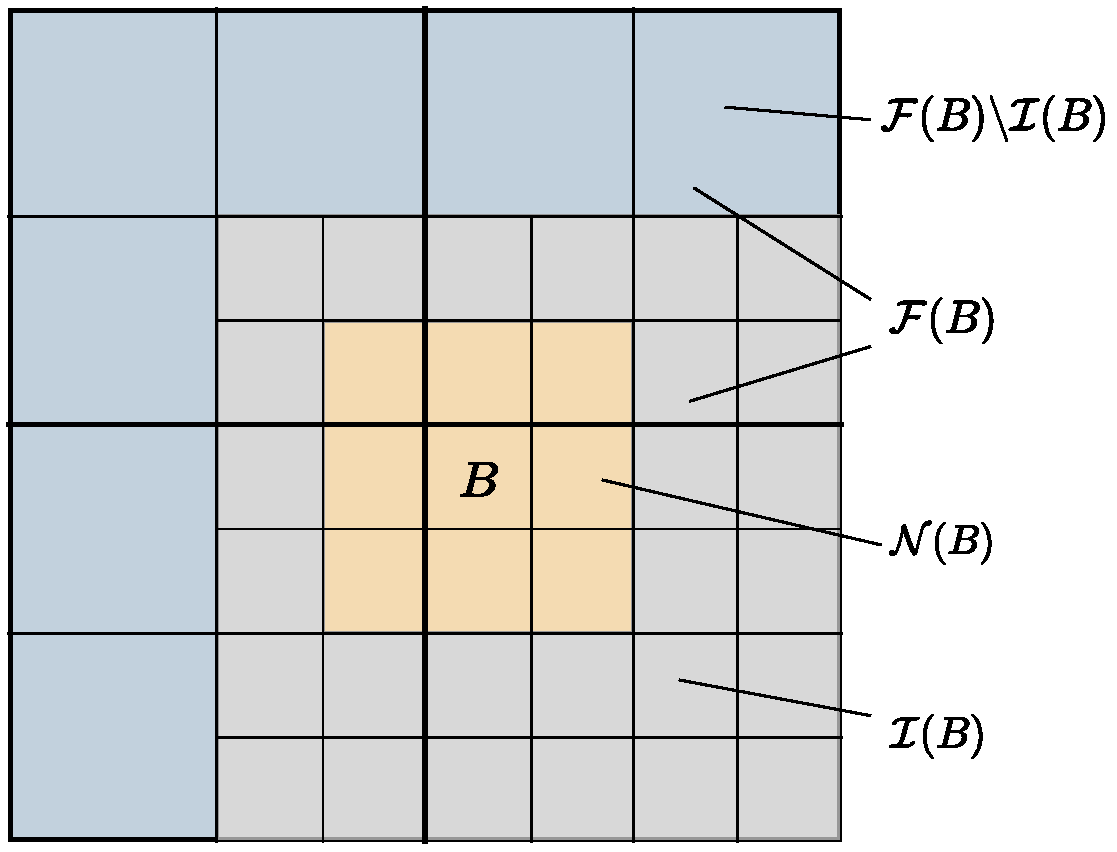
\includegraphics[width=0.8\linewidth]{near_far_decomposition.pdf}
    \caption{An example of a 3-level quadtree.}
    \label{fig:near_far_decomp}
\end{figure}

To construct the octree, we first create a cube that encloses all bodies and then recursively subdivide the domain until each cube at the finest level only contains a constant number of bodies.
Figure \ref{fig:near_far_decomp} depicts a 3-level quadtree.
The potentials of targets in the node $B$ consists of three contributions: the influence from sources in the near-field of $B$: $\mathcal{N}(B)$, in the interaction list of $B$: $\mathcal{I}(B)$ and in the rest of the domain.
$B$'s near-field includes $B$ and its neighbors, where the interactions are computed exactly.
The remaining domain is in $\mathcal{F}(B)$, $B$'s far-field.
In $\mathcal{F}(B)$, the nodes that are the children of $B$'s parent's neighbors but are not adjacent to $B$ compose $\mathcal{I}(B)$, the interaction list of $B$, whose contributions to $B$ are approximated by low-rank methods.
The contributions from the rest of the far-field are approximated at coarser levels via $B$'s ancesters.

The classic \fmm \cite{greengard1987fast, cheng1999fast} relies on truncated analytical expansions to approximate far-field interactions, whereas its kernel-independent variant \cite{ying2004kernel} uses equivalent densities (charges) instead.
In KIFMM, each node is associated with upward and downward equivalent densities (see Figure \ref{fig:multipole_local}), the analog of multipole and local expansion in analytical \fmm.
The upward equivalent densities $q^{B,u}$ are used to approximate the influence of sources in $B$ on targets in $\mathcal{F}(B)$;
the downward equivalent densities $q^{B,d}$ are used to approximate the influence of sources in $\mathcal{F}(B)$ on sources in $B$.
To find these densities, we match the potential of equivalent densities to the potential of actual sources at the check surfaces:
%
\begin{align}
    \sum_{\mathbf{y}_{j} \in B} g\left(\mathbf{x}_{i}^{B,u}, \mathbf{y}_{j}\right) q_{j} &= \sum_{j} g\left(\mathbf{x}_{i}^{B,u}, \mathbf{y}^{B,u}_{j}\right) q^{B,u}_{j}, \quad \forall i  \\
    \sum_{\mathbf{y}_{j} \in \mathcal{F}(B)} g\left(\mathbf{x}_{i}^{B,d}, \mathbf{y}_{j}\right) q_{j} &= \sum_{j} g\left(\mathbf{x}_{i}^{B,d}, \mathbf{y}^{B,d}_{j}\right) q^{B,d}_{j}, \quad \forall i
    \label{eq:multipole_local}
\end{align}
%
, and then solve the linear systems for $\{q^{B,u}_{j}\}$ and $\{q^{B,d}_{j}\}$.
$\mathbf{x}_{i}^{B}$ and $\mathbf{y}_{j}^{B}$ denote the discretization points of the check surface and equivalent surface of $B$ respectively.

\begin{figure}
    \centering
    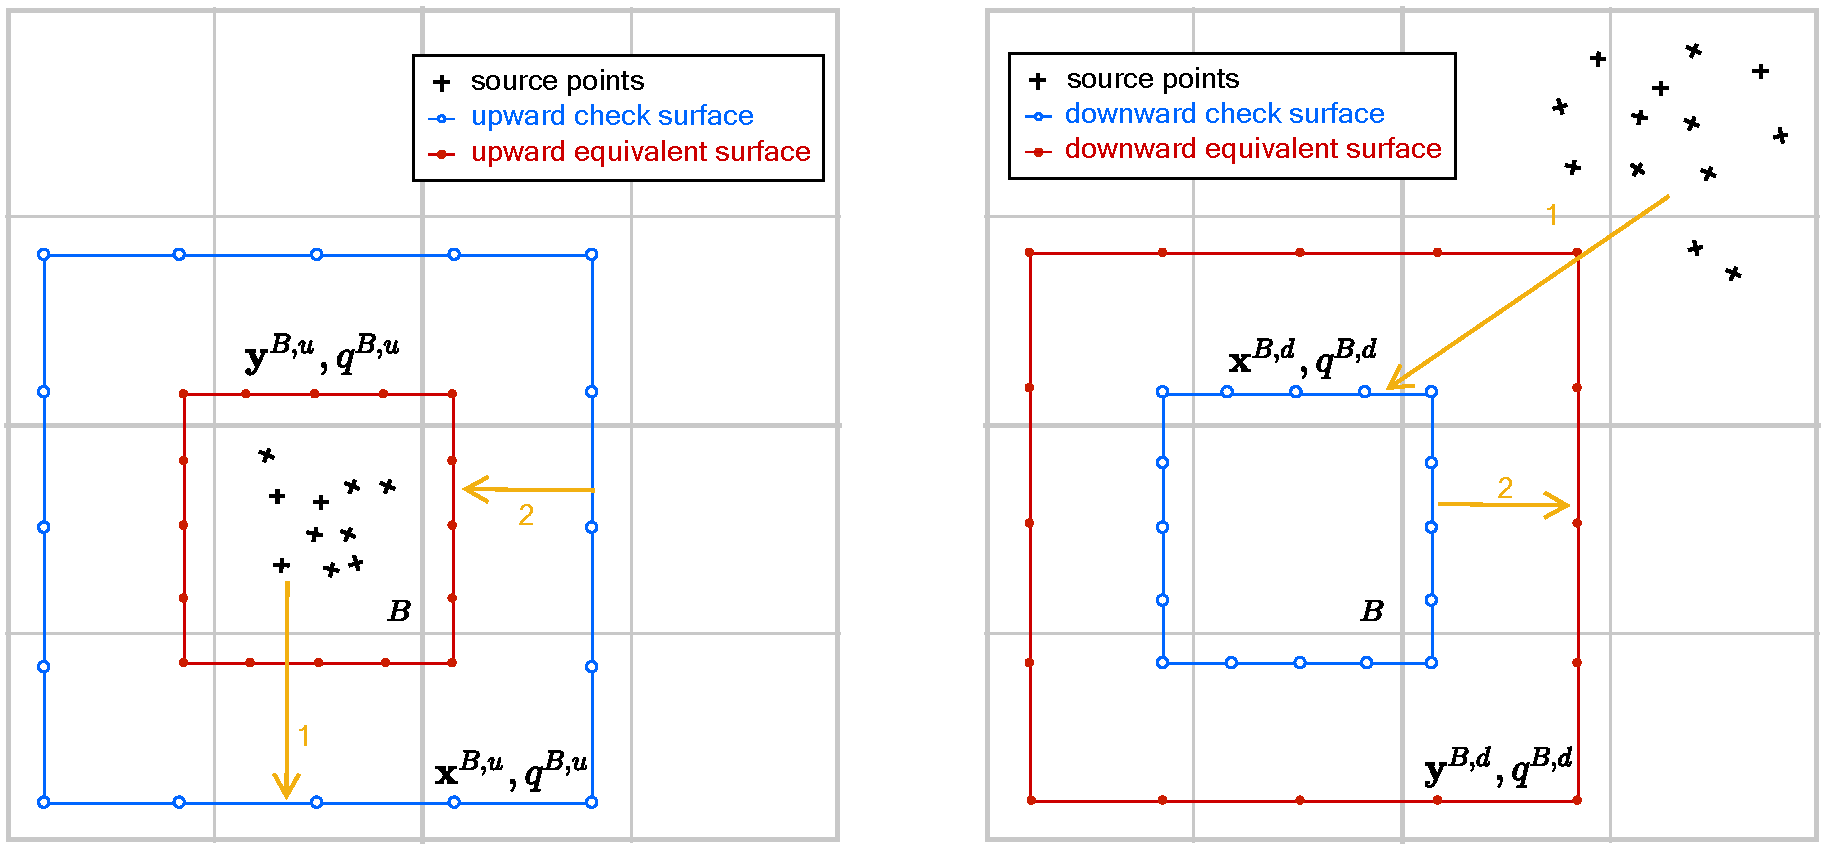
\includegraphics[width=\linewidth]{multipole_local_expansion.pdf}
    \caption{Multipole expansion (left) and local expansion (right) in KIFMM.}
    \label{fig:multipole_local}
\end{figure}

The algorithm also defines the following operators:
%
\begin{itemize}
    \item particle-to-multipole (P2M): For a leaf node $B$, compute $B$'s upward equivalent densities, \ie multipole expansion, from the sources in $B$. (Figure \ref{fig:multipole_local} left)
    \item multipole-to-multipole (M2M): For a non-leaf node $B$, evaluate $B$'s multipole expansion based on the multipole expansions of all $B$'s children. (Figure \ref{fig:translations} left)
    \item multipole-to-local (M2L): For a node $B$, evaluate $B$'s downward equivalent densities, \ie local expansion, by using the multipole expansions of all nodes in $\mathcal{I}(B)$. (Figure \ref{fig:translations} middle)
    \item local-to-local (L2L): For a non-leaf node $B$, add the contribution of $B$'s local expansion to the local expansions of $B$'s children. (Figure \ref{fig:translations} right)
    \item local-to-particle (L2P): For a leaf node $B$, evaluate $B$'s local expansion at the locations of targets in $B$.
    This step adds all far-field contribution to the potentials of targets in $B$. 
    \item particle-to-particle (P2P): For a leaf node $B$, evaluate the potential induced by all sources in $\mathcal{N}(B)$ directly.
\end{itemize}
%
As indicated by the arrows in Figure \ref{fig:translations}, translation operators in KIFMM share the same procedure: (1). evaluating the potentials on the check surface and (2). solving the equation arising from matching the potentials for the equivalent densities.

Figure \ref{fig:fmm_sketch} outlines the complete \fmm algorithm.
During the upward pass, we compute P2M at all leaf nodes and perform M2M in post-order tree traversal.
Next, we compute M2L for all nodes.
Finally, we compute L2L in pre-order tree traversal, and perform L2P and P2P at all leaf nodes during the downward pass.

\begin{figure*}
    \centering
    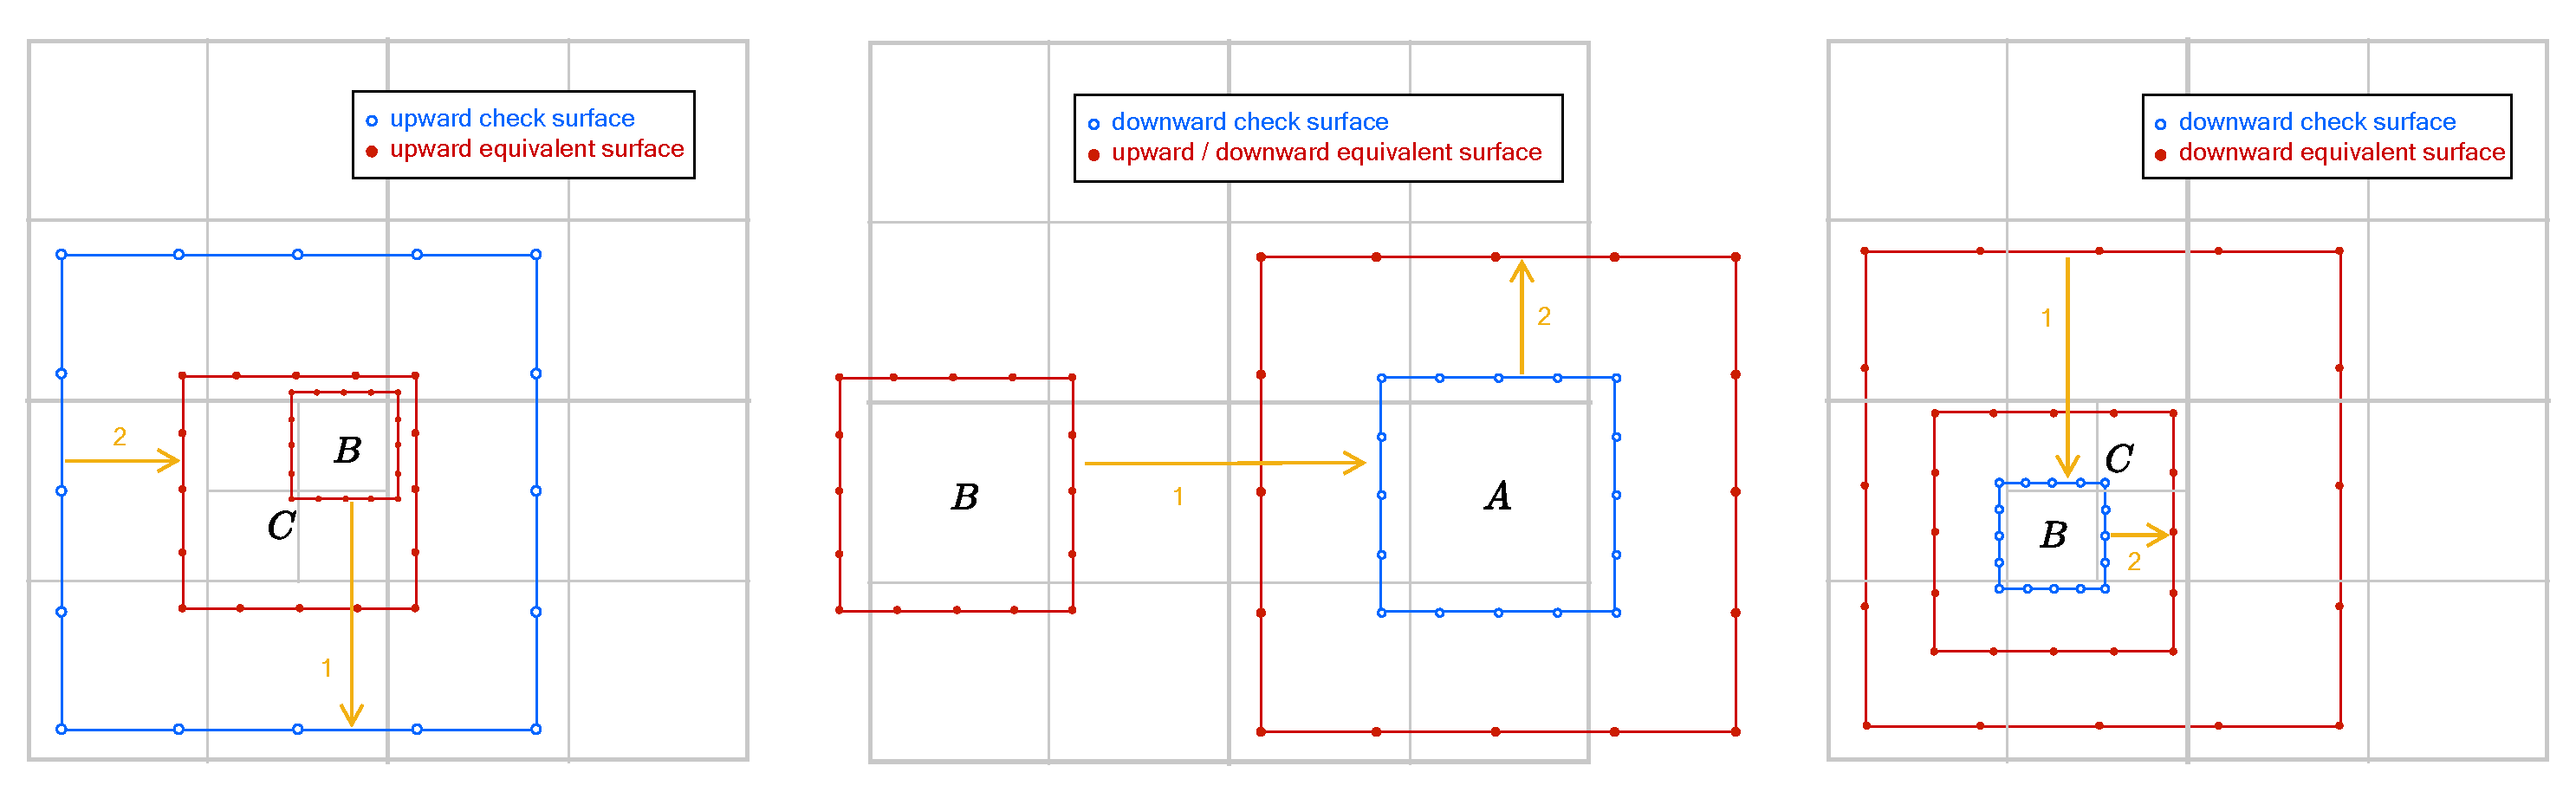
\includegraphics[width=\linewidth]{translations.pdf}
    \caption{M2M (left), M2L (middle) and L2L (right) operators in KIFMM. Node $C$ is the parent of $B$, and node $A$ is in the interaction list of $B$.}
    \label{fig:translations}
\end{figure*}

\begin{figure}
    \centering
    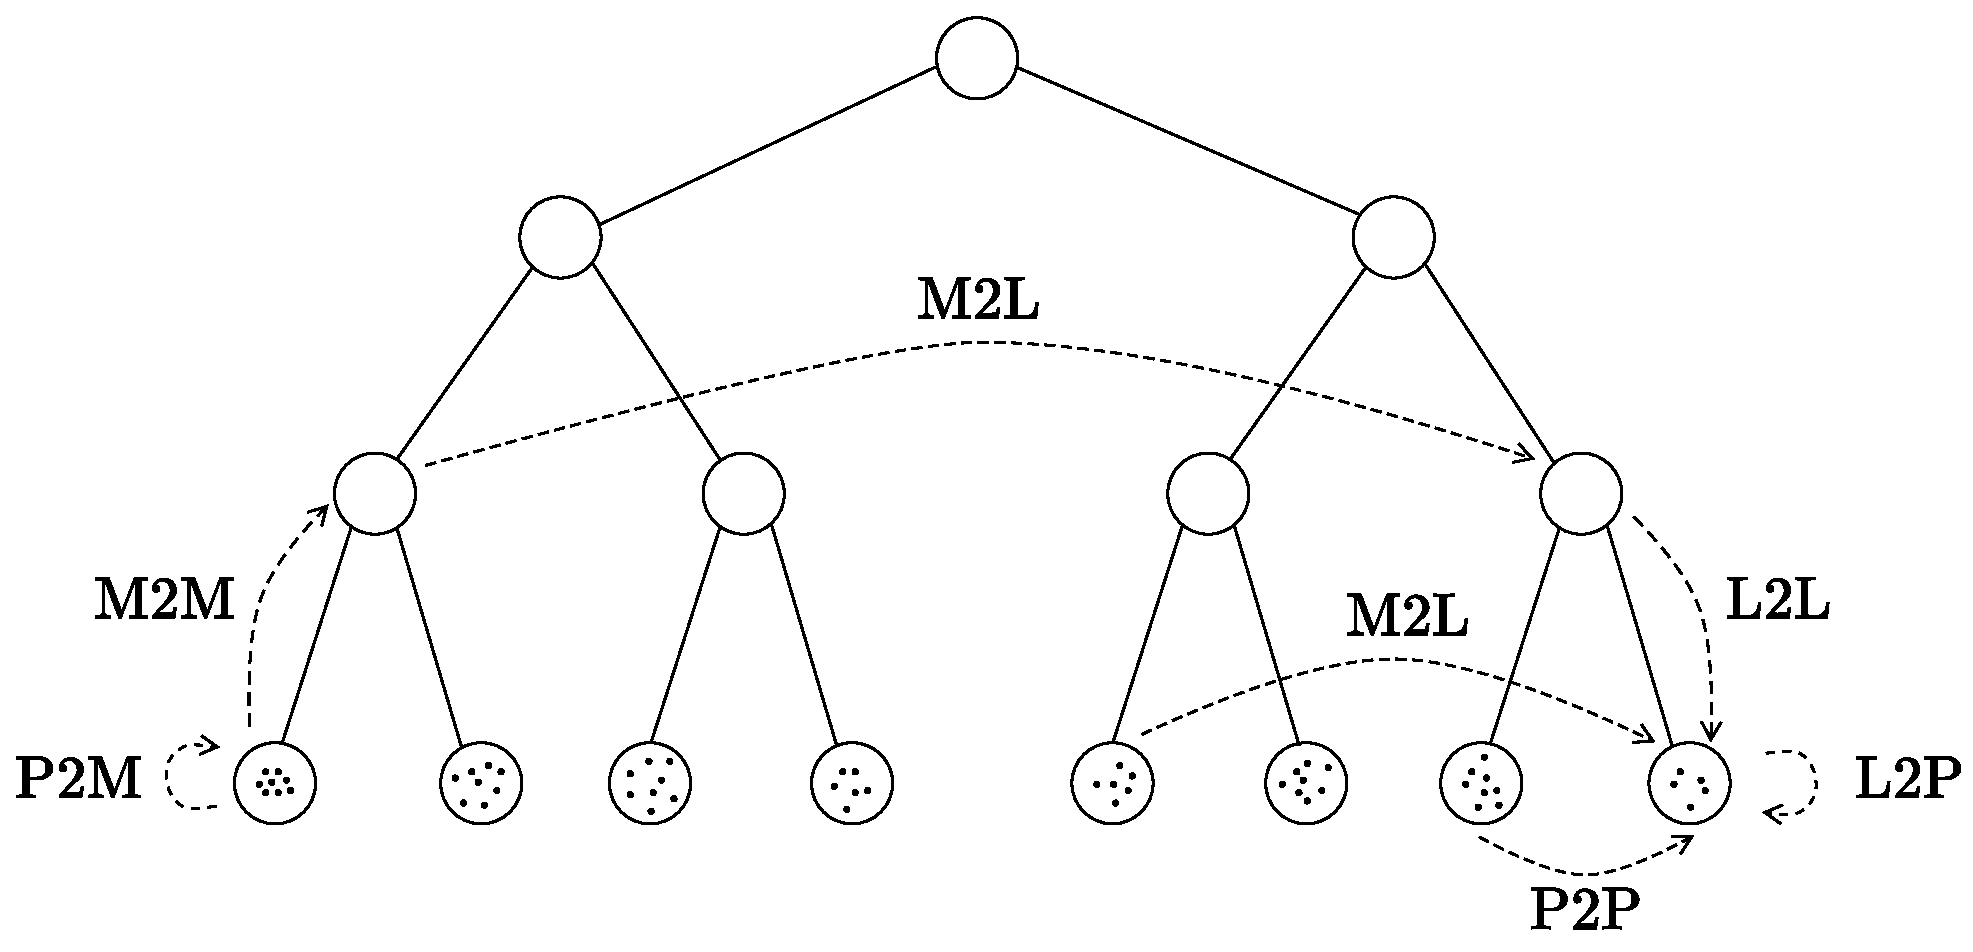
\includegraphics[width=\linewidth]{fmm_sketch.pdf}
    \caption{Sketch of FMM algorithm using a binary tree.}
    \label{fig:fmm_sketch}
\end{figure}

\section{Results}\label{sec:results}
%!TEX root = main.tex
We demonstrate the performance and capability of Bempp-Exafmm via electrostatic simulations, including computing the solvation energy of a Zika virus.
This section presents four types of results. 
The first result explains the behavior of two variants of the mathematical formulation, from the conditioning point of view. 
Second, we show solution verification through two grid-convergence studies: with a spherical molecule (having an analytical solution), and with a real biomolecule (using Richardson extrapolation).
The third type of result looks at performance with problem sizes between 8,000 and 2 million elements, including timings, breakdowns, and computational complexity.
Our final result is a demonstration using a structure with about 1.6 million atoms, the Zika virus, discretized with about 10 million boundary elements.

We ran all experiments on a single CPU node of \textit{Pegasus},\footnote{Pegasus is a Linux cluster at the George Washington University.} equipped with two 20-core Intel Xeon Gold 6148 CPUs running at 3.7 GHz and 192GB RAM.
All runs are based on Bempp-cl version 0.2.2 and Exafmm-t version 0.1.0.
We compiled Exafmm with Intel compiler (version 19.0.5.281) and enabled \texttt{-xHost} option for vectorization.
We used the full GMRES from the SciPy library as our linear solver.

\paragraph{Matrix conditioning of two derivative formulations} \label{result_conditioning}

Section \ref{s:formulation} presents the two formulations to solve the integral equations  \eqref{eq:volume_potential} derived from the Poisson-Boltzmann model of biomolecular electrostatics: 
the \emph{direct}~\cite{YoonLenhoff1990}  and \emph{derivative}~\cite{JufferETal1991} formulations.
The latter is well-known to lead to a better-conditioned matrix.
Its most common solution method finds the potential and its derivative in the interior of the boundary via equations \eqref{eq:juffer}, but an alternative is to solve for the exterior fields via \eqref{eq:lu}.
Bempp unfetters the user to experiment with these variants of the boundary element solution method, editing just a few lines of Python.
We could easily try both the interior and exterior versions of the derivative formulation, whereas previous publications opted for one method and used it throughout.
The programming effort required to implement a second formulation would have been a good reason.
In our experiments, the exterior version used by Lu and coworkers~\cite{LuETal2006,LuETal2009,ZhangETal2019} took about half as many iterations to converge than the interior version---a sizable advantage.
This led us to study the properties of the two variants of the derivative formulation in more detail.
The results in this section aim to give a simple explanation for the different numerical behavior of the two methods.
Our ability to explore and explain this issue showcases the power of interactive computing with a high-productivity software platform, like that provided by Bempp-Exafmm.

GMRES methods have an intricate convergence behavior \cite{mark1999a}.
Heuristically, if the eigenvalues are clustered with the cluster being sufficiently far away from the origin, we expect fast convergence of GMRES to the desired solution.
Figures \ref{fig:derivative_interior_eig} and \ref{fig:derivative_exterior_eig} show the eigenvalues of the interior and exterior derivative formulations, respectively, on the complex plane.
With the interior formulation, eigenvalues cluster around two points, while eigenvalues cluster around only one point with the exterior formulation.

The difference is due to the diagonal of the corresponding system of integral equations.
In the case of the interior formulation, the associated left-hand side operator takes the form
$$
\begin{bmatrix}\frac{1}{2}(1 + \frac{\epsilon_2}{\epsilon_1})I & 0 \\ 0 & \frac{1}{2}(1 + \frac{\epsilon_1}{\epsilon_2})I
\end{bmatrix} + \mathcal{C}_{int},
$$
where $\mathcal{C}_{int}$ is a compact operator on sufficiently smooth domains.\footnote{On smooth domains the single-layer, double-layer and adjoint double-layer operators are compact operators.
Furthermore, the difference of the hypersingular operators is compact \cite{Hiptmair2006-om}.}
The eigenvalues of the interior derivative operator hence accumulate at the points $\frac{1}{2}(1 + \frac{\epsilon_2}{\epsilon_1})$ and $\frac{1}{2}(1 + \frac{\epsilon_1}{\epsilon_2})$.
In contrast, the exterior derivative operator has the form
$$
\begin{bmatrix}\frac{1}{2}(1 + \frac{\epsilon_1}{\epsilon_2})I & 0 \\ 0 & \frac{1}{2}(1 + \frac{\epsilon_1}{\epsilon_2})I
\end{bmatrix} + \mathcal{C}_{ext},
$$
where $\mathcal{C}_{ext}$ is again a compact operator.
We now only have one accumulation point, namely $\frac{1}{2}(1 + \frac{\epsilon_1}{\epsilon_2})$.
Unless $\epsilon_1\approx \epsilon_2$ we therefore expect the eigenvalues to be much closer together than in the interior derivative case and therefore the GMRES convergence to be faster for the exterior derivative formulation.

We want to emphasize that the above argument is valid for the continuous operators. Under discretization, the resulting eigenvalue problem is of the form $A\mathbf{x}=\lambda M\mathbf{x}$ (or equivalently $M^{-1}A\mathbf{x}=\lambda \mathbf{x}$, where $A$ is the $2\times 2$ block operator associated with the Galerkin discretization of the integral operator system and $M = \text{diag}(\hat{M}, \hat{M})$ is a block diagonal mass matrix, where the matrix $\hat{M}$ is the matrix containing the surface inner products $\int_{\Gamma}\psi_i(\mathbf{r})\phi_j(\mathbf{r})ds(\mathbf{r})$ for test functions $\psi_j$ and trial functions $\phi_i$ (which are both chosen as continuous, piecewise linear basis functions in this paper). The mass-matrix preconditioned linear system of equations to solve has the form $M^{-1}A\mathbf{x} = M^{-1}\mathbf{b}$ for vector of unknowns $\mathbf{x}$ and right-hand side $\mathbf{b}$ and Figures \ref{fig:derivative_interior_eig} and \ref{fig:derivative_exterior_eig} show the eigenvalues of $M^{-1}A$ for the interior and exterior Juffer formulation. In practice, the action of $M^{-1}$ can be computed through a sparse LU decomposition of $M$. However, for problems with millions of unknowns this is becoming expensive. We have therefore chosen a simple mass lumping approach, in which we substitute $M$ by a diagonal matrix, where each diagonal entry is the sum of the corresponding row values of $M$. This diagonal matrix can then be trivially inverted. In our experiments the mass lumping only led to a modest increase in the number of iterations compared to using the full mass matrix $M$.

In each of the following studies, we present two sets of results: one from using the exterior derivative formulation with the lumped mass preconditioner, and the other from using the direct formulation with a block-diagonal preconditioner presented by Altman and co-workers \cite{AltmanBardhanWhiteTidor2009}.


\begin{figure*}
    \begin{center}
        \subfloat[][]{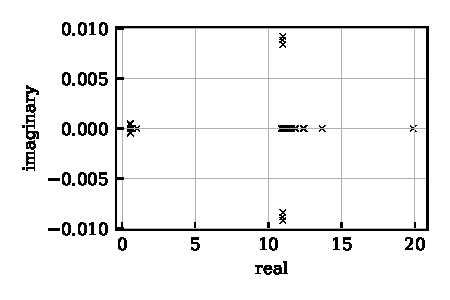
\includegraphics[width=0.4 \textwidth]{derivative_interior_eig.pdf}
        \label{fig:derivative_interior_eig}}\qquad
        \subfloat{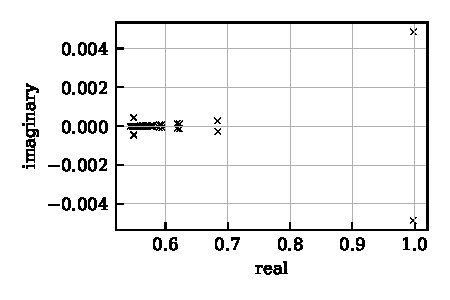
\includegraphics[width=0.4 \textwidth]{derivative_exterior_eig.pdf}
        \label{fig:derivative_exterior_eig}}
    \end{center}
    \caption{Eigenvalues of the system matrix of the derivative formulation for interior field (\textbf{a}) and for exterior field (\textbf{b}).
    }
\end{figure*}

\paragraph{Mesh refinement study using a spherical molecule} \label{result_convergence_sphere}

As a form of solution verification with the Bempp-Exafmm software, we completed two mesh-refinement studies.
The first used a spherical molecule with an off-center charge, for which we have an analytical solution.
In the next sub-section, we present a mesh-refinement study with a real molecule of biological relevance.
Figure \ref{fig:sketch_sphere_convergence} depicts the problem setup for the current case:
a spherical molecule of radius 4 \AA\ and relative permittivity $\epsilon_1 = 4$, with a unit charge located at $(1,1,1)$.
The solvent region has the relative permittivity of water ($\epsilon_2 = 80$), and a salt concentration of $150$mM $(\kappa = 1/8\ {\si{\angstrom}}^{-1})$.
Other simulation parameters are listed in Table \ref{tab:convergence}.
With an expansion order of 10, our \fmm achieved 9 digits of accuracy.
We computed the solvation energy of this molecule using $5$ different meshes, obtained using a constant refinement factor of 4.

\begin{table}[]
    \centering
    \begin{tabular}{lc}
    \hline
    \gmres tolerance          & $10^{-7}$ \\
    \# regular quadrature points  & 6    \\
    \fmm expansion order      & 10   \\
    \fmm $\ncrit$             & 500  \\
    \hline  \vspace{0.3 cm}
    \end{tabular}

    \begin{tabular}{cc}
    number of elements & mesh density ($\#/{\si{\angstrom}}^2$) \\
    \hline
    3032               & 1                                       \\
    6196               & 2                                       \\
    12512              & 4                                       \\
    25204              & 8                                       \\
    50596              & 16                                     
    \end{tabular}
    \caption{Simulation parameters for the grid-refinement studies (top); mesh sizes/densities used in the grid refinement study on 5PTI. Mesh densities measured as number of elements per square Angstrom.}
    \label{tab:convergence}
\end{table}

Kirkwood's derivation \cite{kirkwood1934theory} allows us to compute the analytical solution for the solvation energy in this case, to compare with the numerical result: $-12.258363$ [kcal/mol].
Figure \ref{fig:sphere_convergence} shows the error in the solvation energy, converging at the expected rate of $1/N$ for both formulations.
The observed order of convergence is 1.001 for the direct formulation and 0.999 for the derivative formulation, using the middle three values.

\paragraph{Mesh refinement study using 5PTI} \label{result_convergence_5PTI}

Next, we tested our software using a real biomolecule: bovine pancreatic trypsin inhibitor (PDB code 5PTI), whose structure \cite{wlodawer1984structure} is shown in Figure \ref{fig:5PTI_structure}.
We parameterized the molecule with \texttt{pdb2pqr}~\cite{DolinskyETal2004} and the \texttt{charmm} force field, and then computed the solvation energy using 5 meshes with the element density ranging from 1 to 16 (Table \ref{tab:convergence}).
This test used the same parameters listed in Table \ref{tab:convergence}, which are fine enough to reveal the discretization error.
Since an analytical solution is not available for this geometry, we obtained the reference values for error estimation via Richardson extrapolation.
The estimated relative error with the finest mesh is 1.2\% with the direct formulation, and 1.5\% with the derivative formulation.



Figure \ref{fig:5PTI_convergence} shows that the error of the computed solvation energy for 5PTI converges linearly with respect to $N$.
The observed order of convergence is 1.156 for the direct formulation and 1.038 for the derivative formulation, using the middle three values.
Both convergence results provide solution verification, and are evidence that our software solves the mathematical model correctly.

\begin{figure*}
        \centering
     \subfloat[][Sphere with an off-center unit charge at $(1,1,1)$.]{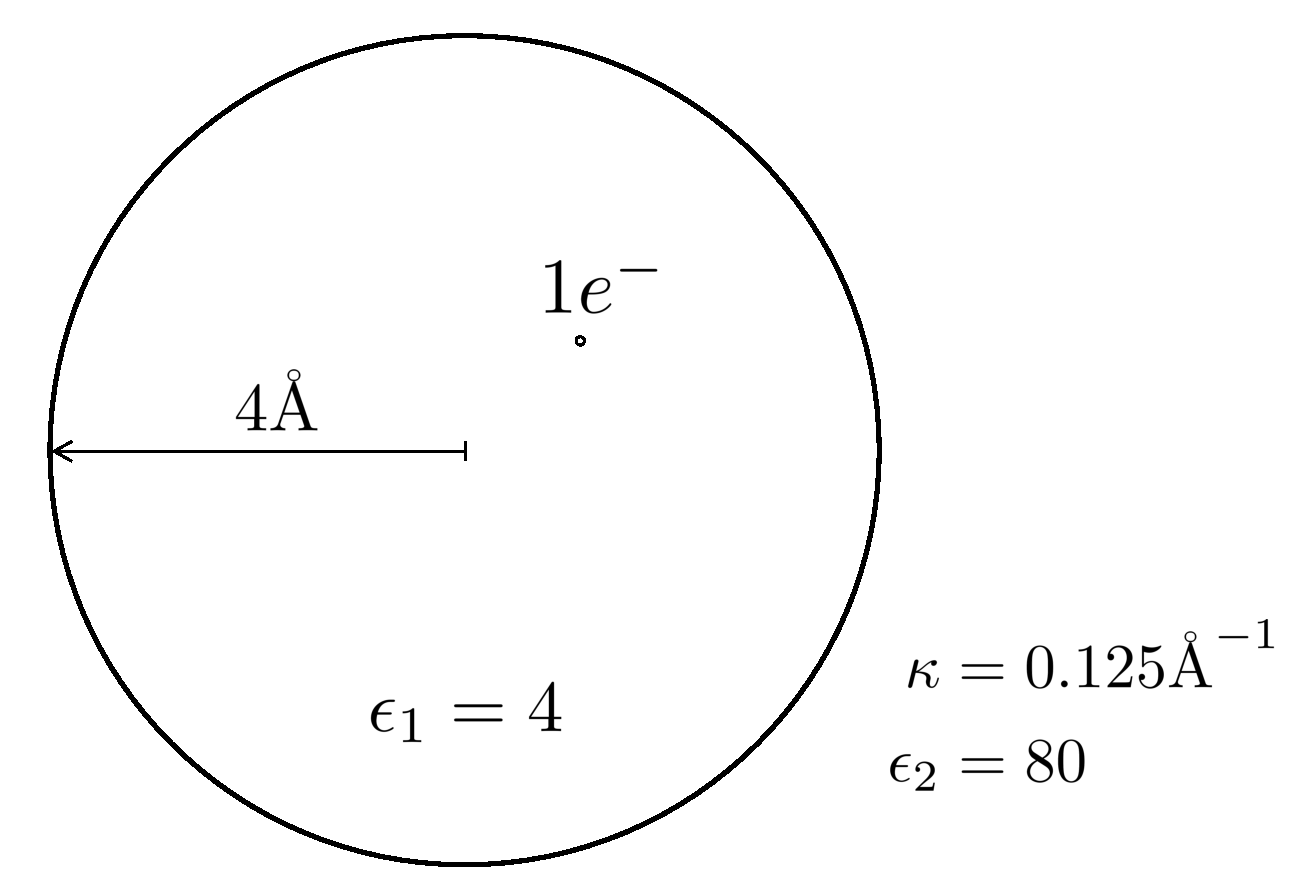
\includegraphics[width=0.4 \textwidth]{sketch_sphere_convergence.pdf}
        \label{fig:sketch_sphere_convergence}}\quad
     \subfloat[][Structure of 5PTI.]{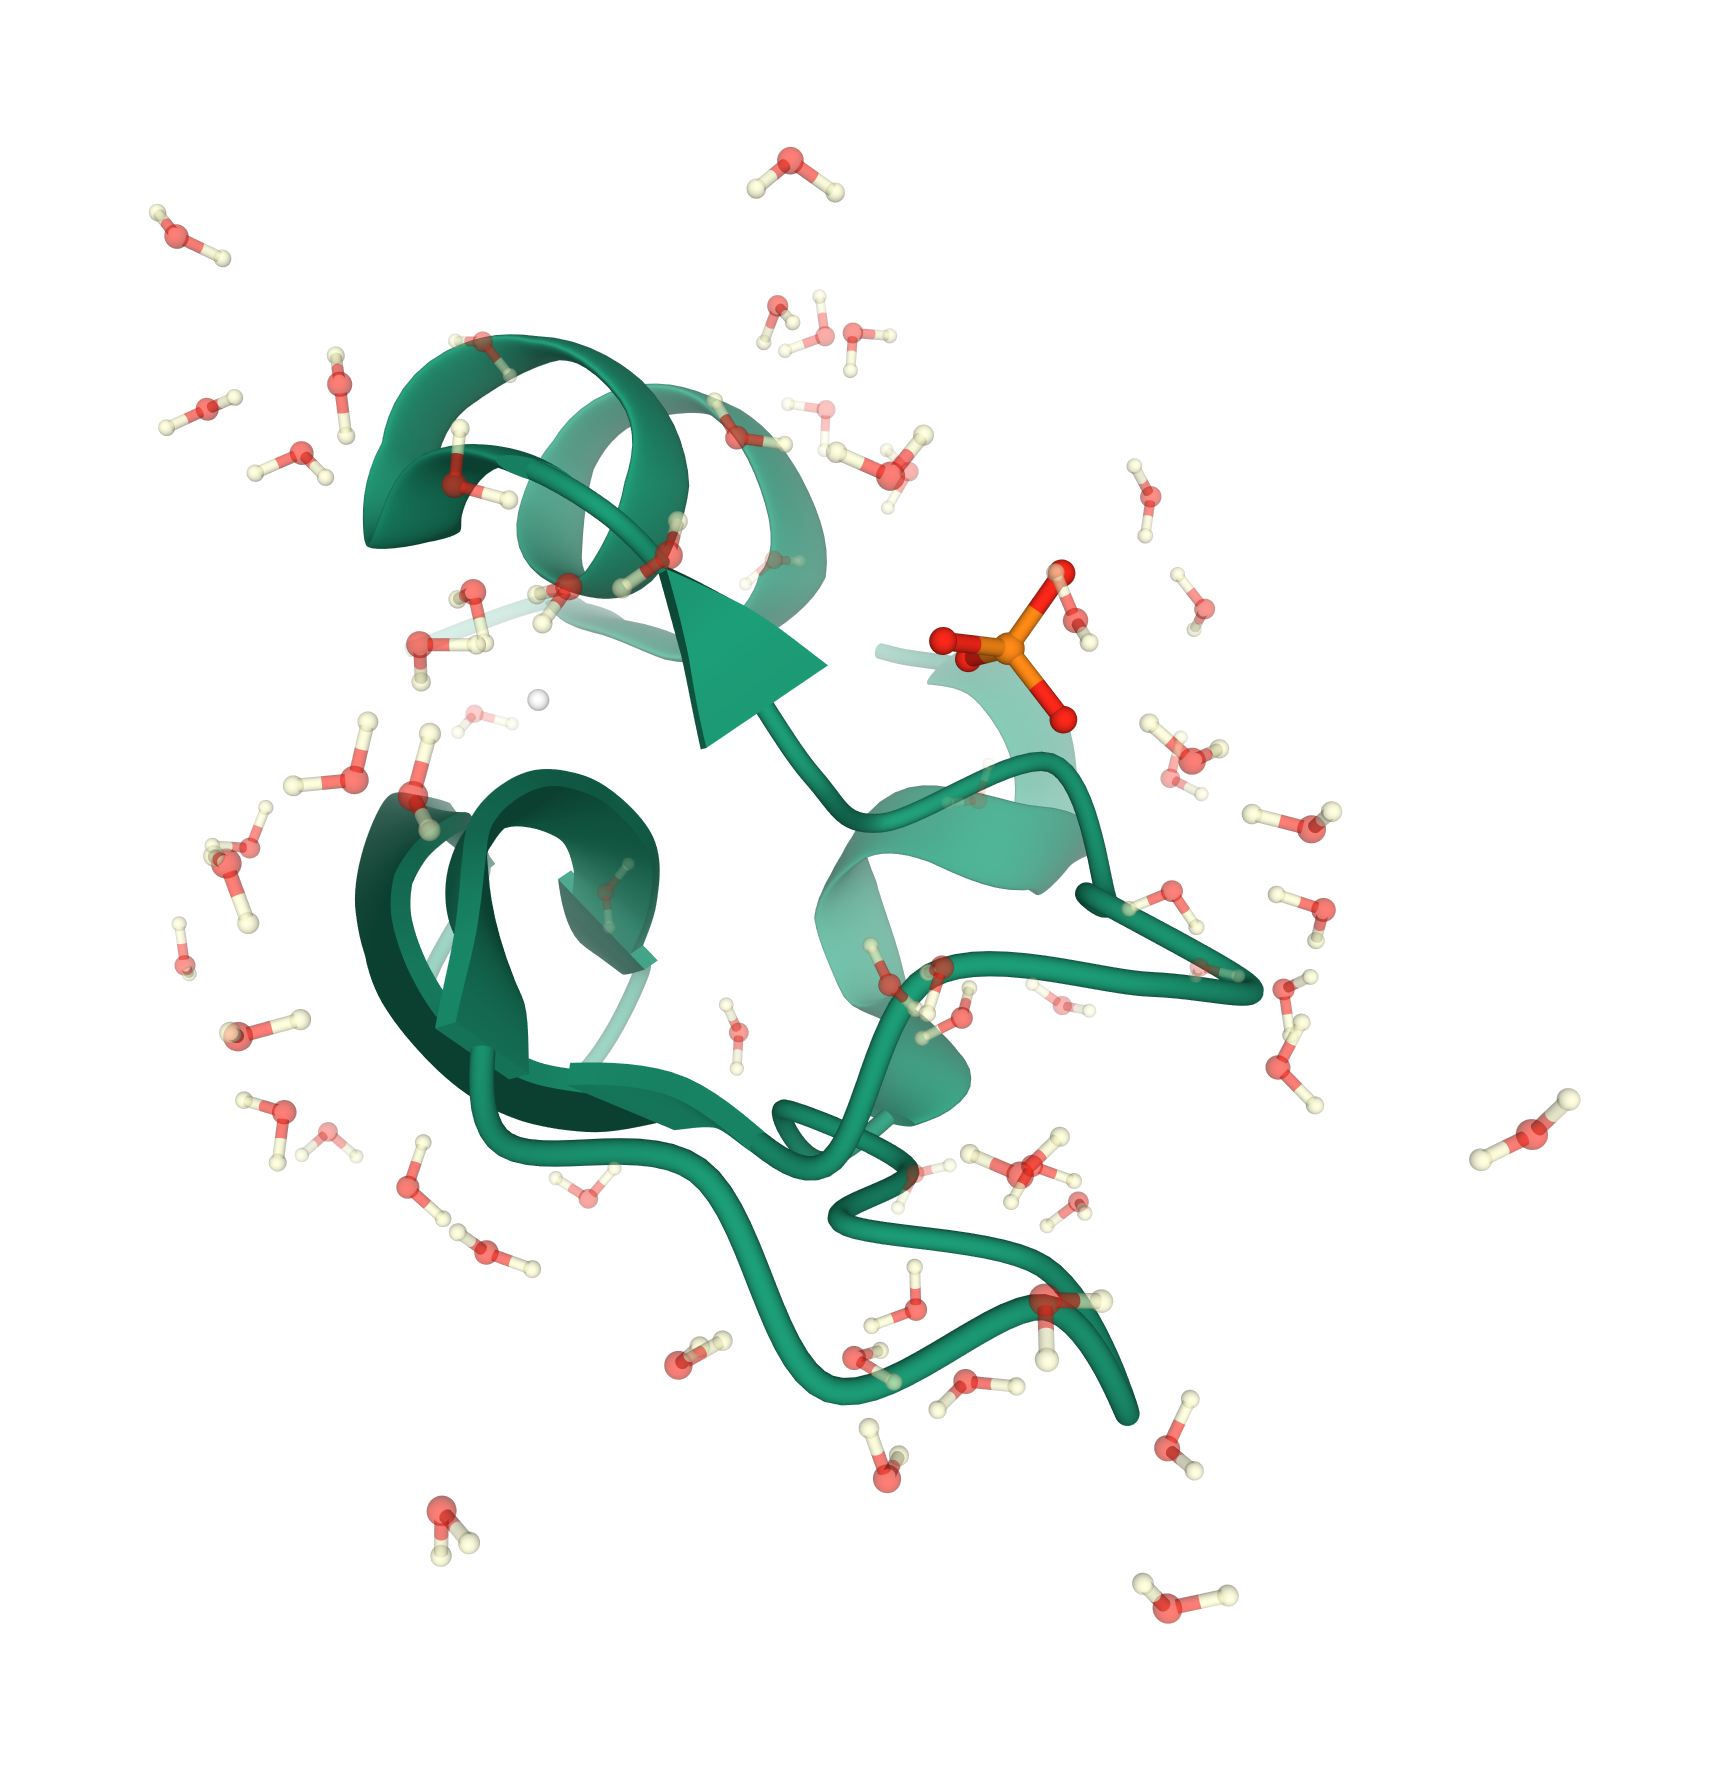
\includegraphics[width=0.35 \textwidth]{5PTI.png}
        \label{fig:5PTI_structure}}\\
     \subfloat[][]{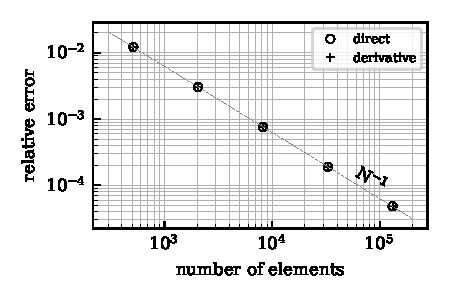
\includegraphics[width=0.4 \textwidth]{sphere_convergence.pdf}
        \label{fig:sphere_convergence}}
     \subfloat[][]{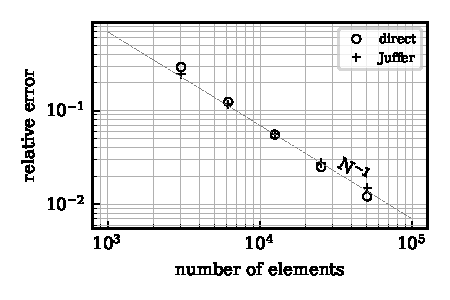
\includegraphics[width=0.4 \textwidth]{5PTI_convergence.pdf}
        \label{fig:5PTI_convergence}}
    \caption{Mesh refinement studies using a spherical molecule and a real biomolecule: bovine pancreatic trypsin inhibitor (PDB code 5PTI).
    \textbf{c}, Mesh convergence study on a spherical molecule with an off-center charge, using both direct formulation and derivative formulation. The error on the solvation energy with respect to the analytical solution is plotted for five meshes:
    the sphere discretized with 512, 2048, 8192, 32768 and 131072 boundary elements.
    \textbf{d}, Mesh convergence study of the solvation energy of bovine pancreatic trypsin inhibitor (PDB code 5PTI), using both direct formulation and derivative formulation.
    The error is with respect to the extrapolated solution using Richardson extrapolation.
    }
\end{figure*}


\paragraph{Performance study with direct and derivative formulations} \label{result_performance}

In this sub-section, we investigate the computational performance of Bempp-Exafmm using a spherical molecule.
The sphere has a radius of 1, and 100 charges are placed randomly inside, representing the atoms in the solute.
We used the same dielectric constants and salt concentration as in previous grid-convergence studies.
Other simulation parameters are listed in Table \ref{tab:sim_params_performance}.

\begin{table}[]
    \centering
    \begin{tabular}{lc}
    \hline
    \gmres tolerance          & $10^{-4}$ \\
    \# regular quadrature points  & 6    \\
    \fmm expansion order      & 5   \\
    \fmm $\ncrit$             & 500  \\
    \hline
    \end{tabular}
    \caption{Simulation parameters used in the performance study for a spherical molecule.}
    \label{tab:sim_params_performance}
\end{table}

To cover a wide range of problem sizes, we used five surface discretizations, with the number of elements ranging from 8 thousand to 2 million.
Table \ref{tab:sphere_time} presents the assembly time, the solution time and the number of iterations to converge in each case for both formulations.
The assembly time includes the time to pre-compute the \fmm invariant matrices, create sparse and singular assemblers and calculate preconditioners.
The algebraic convergence shows that the condition number grows as the problem size increases with the direct formulation, while it remains at the same level with the derivative formulation.

\begin{table*}[]
    \centering
    \begin{tabular}{c|cccc|cccc}
                                                                 & \multicolumn{4}{c|}{direct}                                                                                                                                                                       & \multicolumn{4}{c}{derivative}                                                                                                                                                                        \\ \hline
    \begin{tabular}[c]{@{}c@{}}number of\\ elements\end{tabular} & \begin{tabular}[c]{@{}c@{}}total\\ time (s)\end{tabular} & \begin{tabular}[c]{@{}c@{}}assembly\\ time (s)\end{tabular} & \begin{tabular}[c]{@{}c@{}}GMRES\\ time (s)\end{tabular} & \# iterations & \begin{tabular}[c]{@{}c@{}}total\\ time (s)\end{tabular} & \begin{tabular}[c]{@{}c@{}}assembly\\ time (s)\end{tabular} & \begin{tabular}[c]{@{}c@{}}GMRES\\ time (s)\end{tabular} & \# iterations \\ \hline
    8192                                                         & 14.0                                                     & 5.4                                                         & 8.6                                                      & 20            & 16.1                                                     & 9.6                                                         & 6.5                                                      & 5            \\
    32768                                                        & 35.1                                                     & 11.7                                                        & 23.4                                                     & 24            & 35.5                                                     & 22.2                                                        & 13.3                                                     & 4            \\
    131072                                                       & 144.2                                                    & 32.8                                                        & 111.4                                                    & 34            & 114.7                                                    & 67.2                                                        & 47.5                                                     & 4            \\
    524288                                                       & 675.8                                                    & 121.6                                                       & 554.2                                                    & 51            & 421.3                                                    & 256.3                                                       & 165.0                                                    & 4            \\
    2097152                                                      & 3159.8                                                   & 483.3                                                       & 2676.5                                                   & 70            & 1592.1                                                   & 1011.6                                                      & 580.5                                                    & 4           
    \end{tabular}
    \caption{Assembly and solution times of calculating the solvation energy of a spherical molecule with 100 random charges inside, using the direct and derivative (exterior) formulations.
    6 regular quadrature points were used per element and the \fmm expansion order was set to 5.}
    \label{tab:sphere_time}
\end{table*}

In our implementation, each iteration in direct formulation requires $8$ \fmm evaluations, whereas each iteration in the derivative formulation requires 19, making it more than twice as expensive.
That explains why the direct formulation leads to a shorter solution time (\gmres time), despite a slower convergence, in the two smaller cases.
For larger problem sizes, faster convergence in the derivative formulation offsets the larger cost per iteration.

As for the assembly time, the derivative formulation is about $2\times$ slower, since it needs to construct twice as many operators as the direct formulation.
In addition, the two hypersingular operators make it even more involved.
Figure \ref{fig:sphere_assembly_time} shows the linear scaling of the assembly time with respect to $N$.

Next, we want to confirm that the time complexity of mat-vecs in \gmres is also $\mathcal{O}(N)$.
The Poisson equation requires \fmm with Laplace kernel and the linearized Poisson-Boltzmann equation requires \fmm with Yukawa kernel.
As we mentioned before, each iteration involves multiple \fmm evaluations: 4 Laplace {\fmm}s and 4 Yukawa {\fmm}s for the direct formulation, 8 and 11 for the derivative formulation.
We averaged the time spent on 1 Laplace \fmm and 1 Yukawa \fmm respectively using direct formulation, and plotted it with respect to $N$ in Figure \ref{fig:sphere_fmm}.
Using an \fmm order of 5, we achieved about 5 digits of accuracy in each mat-vec.
The timings and linear scaling substantiate the efficiency of our \fmm implementation.
In the largest case with over 12 million quadrature points, one Laplace \fmm costs $2.1$s and one Yukawa \fmm costs $5.4$s to compute.

In Bempp, the matrix-vector product has the shape $A\mathbf{x} = P_2^T (G - C)P_1 \mathbf{x} + S \mathbf{x}$ (see Equation \ref{eq:bempp_fmm_matvec}), where the dominant costs are the \fmm evaluation of the Green's function matrix $G$ and the on-the-fly evaluation of the singular correction matrix $C$. Moreover, as stated above for the full $2\times 2$ block system a number of \fmm passes together with corresponding singular corrections need to be performed.
Therefore, the \gmres time reported here consists of \fmm time, singular correction time, as well as the time spent on other steps in the \gmres algorithm.
Figure \ref{fig:sphere_gmres_direct} and \ref{fig:sphere_gmres_derivative} show the time breakdown of \gmres in percentages.
As problem size increases, \fmm evaluations dominate the solution time.

We also measured the peak memory usage using the GNU time\footnote{Some Linux distributions do not ship with GNU time.} command \texttt{/usr/bin/time -v}.
We observed a linear space complexity as shown in Figure \ref{fig:sphere_memory}.
The largest case, with more than $2$ million elements, requires $36$GB for the direct formulation and $43$GB for the derivative formulation.

\begin{figure*}[t]
\centering
    \subfloat[][Assembly time]{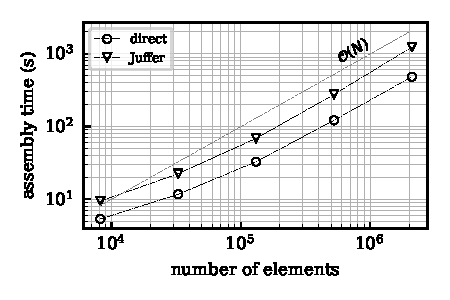
\includegraphics[width=0.33\textwidth]{sphere_assembly_time.pdf}
        \label{fig:sphere_assembly_time}}
   \subfloat[][Average evaluation time.]{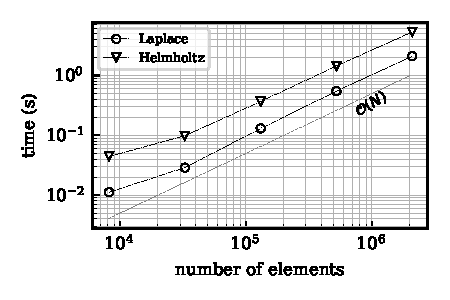
\includegraphics[width=0.33\textwidth]{sphere_fmm.pdf}
        \label{fig:sphere_fmm}}
    \subfloat[][Overall memory consumption in GB.]{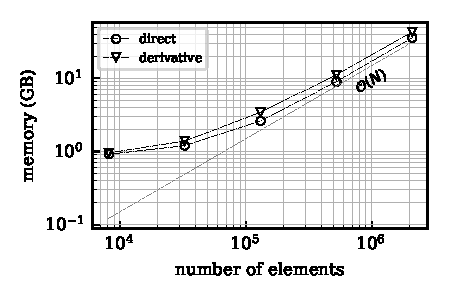
\includegraphics[width=0.33\textwidth]{sphere_memory.pdf}
        \label{fig:sphere_memory}}\\
    \subfloat[][]{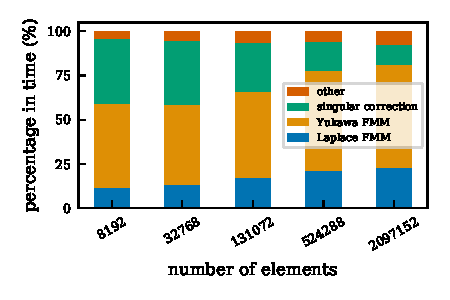
\includegraphics[width=0.4\textwidth]{sphere_gmres_direct.pdf}
        \label{fig:sphere_gmres_direct}}
  \subfloat[][]{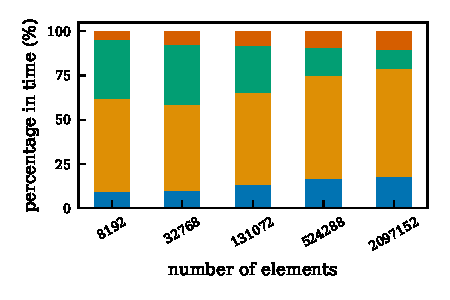
\includegraphics[width=0.4\textwidth]{sphere_gmres_derivative.pdf}
        \label{fig:sphere_gmres_derivative}}
    \caption{Performance on a spherical molecule with 100 random charges inside;
    6 regular quadrature points per element; \fmm expansion order set to 5 to achieve 5 digits of accuracy. Problem size represented by number of elements, $N$. Evaluation time (b) is an average for 1 Laplace \fmm evaluation and 1 Yukawa \fmm evaluation across all iterations in GMRES using direct formulation.
    \textbf{c},\textbf{d}, Time breakdown of \gmres in percentage using direct formulation (\textbf{c}) and derivative formulation (\textbf{d}).}
\end{figure*}

\paragraph{Solvation energy of a Zika virus} \label{result_zika}

Finally, we present a more challenging problem that studies the solvation energy of the Zika virus (PDB code 6CO8), whose structure \cite{sevvana2018refinement} is shown in Figure \ref{fig:6CO8_assembly}.
We downloaded the molecular structure from the Protein Data Bank (PDB), parameterized it with the \texttt{amber} force field, and generated a mesh on the solvent-excluded surface using \texttt{Nanoshaper}.
The prepared structure contains about 1.6 million atoms and our mesh has around 10 million boundary elements, corresponding to between 1 and 2 triangles per square Angstrom.
In this experiment, 3 quadrature points were used for regular Galerkin integrals over disjoint elements.
The \fmm expansion order was set to 4 obtain 4 digits of accuracy in mat-vecs and the tolerance of \gmres was $10^{-4}$.

\begin{table*}[]
    \centering
    \begin{tabular}{c|c|ccccc}
                 & \begin{tabular}[c]{@{}c@{}}$\Delta G_{\mathrm{solv}}$\\ (kcal/mol)\end{tabular} & \begin{tabular}[c]{@{}c@{}}total \\ time (s)\end{tabular} & \begin{tabular}[c]{@{}c@{}}assembly \\ time (s)\end{tabular} & \begin{tabular}[c]{@{}c@{}}GMRES \\ time (s)\end{tabular} & \begin{tabular}[c]{@{}l@{}}memory\\ (GB)\end{tabular} & \# iterations \\ \hline
    direct     & -116587.5                                               & 11005.4                                                   & 1534.5                                                       & 9470.9                                                    & 109.7                                                 & 105           \\
    derivative & -116254.9                                               & 8370.3                                                    & 3553.9                                                       & 4816.4                                                    & 152.0                                                 & 18            
    \end{tabular}
    \caption{Results of computing the solvation energy of a Zika virus with Bempp using both the direct and derivative formulations.
    3 regular quadrature points were used per element and the \fmm expansion order was set to 4.
    To verify our result, we ran the same case with \pygbe using the direct formulation on a workstation with a 24-core CPU.
    The solvation energy computed from \pygbe is -117261.1 [kcal/mol].
    }
    \label{tab:6CO8_result}
\end{table*}

\begin{figure*}
    \subfloat[][]{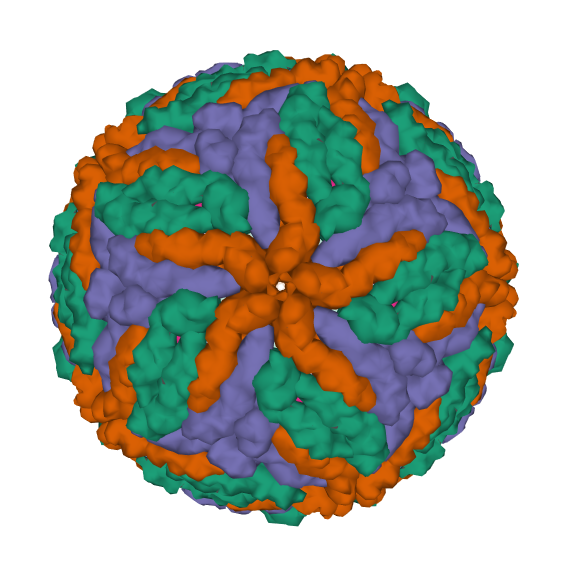
\includegraphics[width=0.25\textwidth]{6CO8_assembly.png}
        \label{fig:6CO8_assembly}}
\subfloat[][]{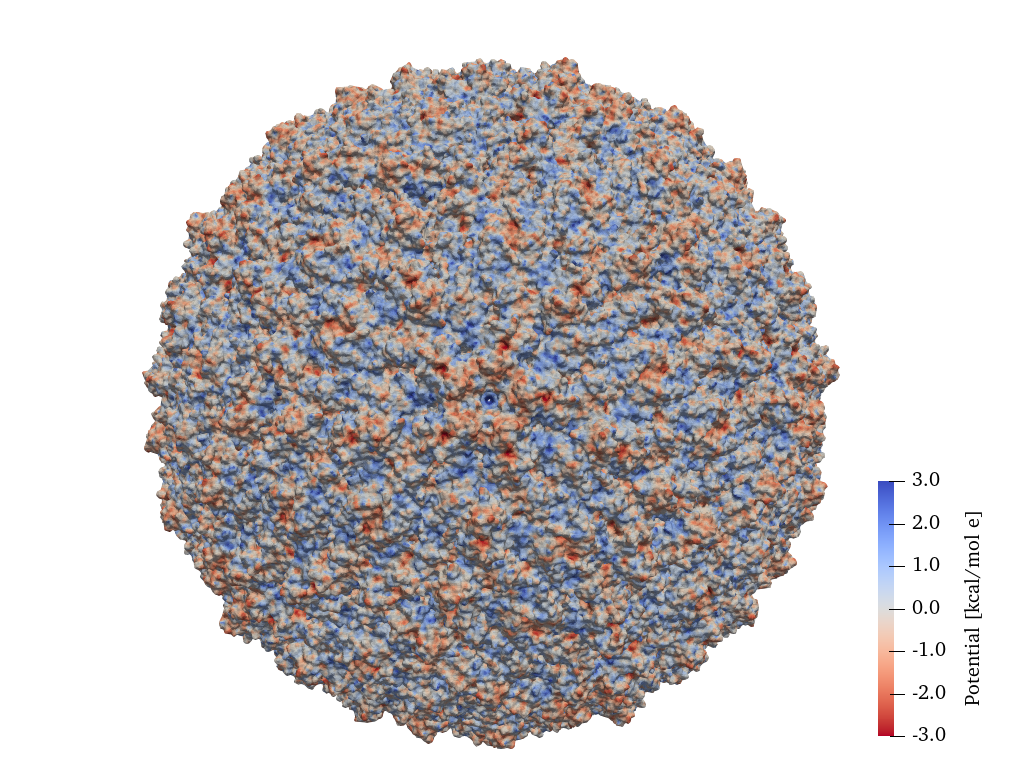
\includegraphics[width=0.75\textwidth]{6CO8_potential.png}
        \label{fig:6CO8_potential}}
    \caption{\textbf{a}, Structure of Zika virus (PDB code 6CO8) in assembly view. Each color indicates a polymer chain.
    \textbf{b}, Surface electrostatic potential of a Zika virus. Visualization generated using ParaView. The starfish pattern seen in the polymer-chain colorization of Figure \ref{fig:6CO8_assembly} is faintly visible in the potential.
    }
\end{figure*}

Table \ref{tab:6CO8_result} summarizes the results and performance.
Again, we confirmed that the derivative formulation yields a well-conditioned system, which converged in 18 iterations and took less than 1.5 hours to solve.
By contrast, the direct formulation took almost twice as long to converge.

In this case, we also verified against \pygbe \cite{cooper2016pygbe}, a Python \bem library for biomolecular electrostatics.
Based on the solvation energy computed from \pygbe: $-117261.1$ [kcal/mol], the relative difference of our result is 0.6\% with the direct formulation and 0.9\% with the derivative formulation.
Figure \ref{fig:6CO8_potential} shows the computed electrostatic potential on the surface.

\paragraph{Reproducibility package}

Besides releasing all our software with an open-source license, we spared no effort to maximize the reproducibility of this work, compiling a ``repro-pack" in a version-control repository.
It contains all raw data from the experiments and a small Python package---\texttt{bempp\_pbs}, to facilitate running PB simulations with Bempp.
\texttt{bempp\_pbs} comprises a collection of scripts, including all post-processing scripts that are necessary to produce every result presented in this section, and driver and utility scripts for different formulations, with which readers can run these cases on their own hardware.
In addition, the ``repro-pack" also provides a Jupyter notebook for each study to generate secondary data and results.
The notebook corresponding to section \ref{result_conditioning} showcases how we could run a simple case of a spherical molecule using two formulations with just a few lines of code, and then compare their conditioning quantitatively with the help of other scientific Python tools.
These supplementary materials are included in our paper's GitHub repository at \href{https://github.com/barbagroup/bempp\_exafmm\_paper/}{https://github.com/barbagroup/bempp\_exafmm\_paper/}, which is also archived on Zenodo at \href{http://doi.org/10.5281/zenodo.4568951}{doi:10.5281/zenodo.4568951}.
We made separate archival deposits of input data (meshes and \texttt{pqr} files ) on the Zenodo service.
The deposit can be downloaded from \href{http://doi.org/10.5281/zenodo.4568768}{doi:10.5281/zenodo.4568768}.


\section{Discussion} \label{sec:discussion}
A Poisson-Boltzmann solver is not something new in itself. They have been around for decades, are available as stand-alone applications and web servers, and come in a variety of implementations, ranging from FD [apbs,delphi,mibpb], to FE[apbs], and BE[afmpb,tabi,pygbe] methods. Moreover, some are integrated into a number of computational workflows that use them for mean field potential visualization [VMD] and free energy calculations [g\_mmpbsa,mmpbsa], usually interfaced through bash or Python scripts.

The modern design of Bempp is built such that high-performance computations are accessible from a high-productivity language. This makes our effort stand out in the current landscape of Poisson-Boltzmann solvers in three ways: interoperability, ease of use, and robustness. 
\begin{enumerate}
\item Interoperability: Bempp is written in Python, and hence, is callable from a Jupyter notebook. This fits naturally in any computational workflow that uses Jupyter notebooks, for example, with openMM [openmm], Biobb [biobb], pytraj [pytraj], or pymol [pymol]. Then, the Jupyter notebook becomes a computational glue across models and scales; no interface script required. 

\item Ease of use: Python and Jupyter notebooks are widely used, even in non-computational settings. Bempp is easily installed through conda, and gives a result in less than 20 lines of code. This, moreover, using parallel and state-of-the-art algorithms in a way that is almost transparent to the user, allowing for large-scale simulations on workstations or small clusters at no extra cost.

Also, there is a thin layer between the application and Bempp, giving a more experienced user access to develop new models, for example, through the FEM-BEM coupling capability of Bempp.

\item Robustness: Bempp is actively developed with high standards of software engineering, such as unit and system testing, continuous integration, etc. Moreover, it was originally designed for scattering problems, impacting a large group of people, well beyond the molecular simulation community. This builds higher trust and reliability of the code, as it is thoroughly tested in a diverse set of applications. Moreover, the software has a better chance to survive in the long term, and any improvements done by people in other domains will have an effect in its use to solve the Poisson-Boltzmann equation. 

\end{enumerate}

There is a large number of popular molecular simulation software designed for different applications, scales, quantities of interest, etc. This led to community-wide efforts, such as BioExcel and MolSSI, that are looking for a common ground between them, as well as promoting good software development practices for robust and easy-to-use codes. This standard is very much aligned with our work.



\bibliography{reference}{}
\bibliographystyle{elsarticle-num}
\end{document}
